\documentclass[10pt]{article}
\usepackage{parskip}
\usepackage[utf8]{inputenc}
\usepackage[left=2.00cm, right=2.00cm, top=2.00cm, bottom=2.00cm]{geometry}
\usepackage[spanish]{babel}
\usepackage{graphicx,subfig}
\usepackage{fancyhdr}
\graphicspath{{Imagenes/}}
\usepackage{enumerate} 
\usepackage{multicol}
\usepackage{tabularx}
\usepackage{amssymb}
\usepackage{adjustbox}
\usepackage{amsmath}
\usepackage{cancel}
\begin{document}


\pagestyle{fancy}
\cfoot{}


%Cabeceras
\rhead{Tarea de Simulacion.}
\lhead{}

%Portada
\begin{titlepage}
	\newgeometry{
		left=25mm,
		right=25mm,
		top=5mm,
		bottom=30mm,
		headheight = 0 mm
	}

	\begin{figure}[t]
		\subfloat{
\includegraphics[width=0.15\textwidth]{Logo_IPN}}
		\hspace{0.6\textwidth}
		\subfloat{
\includegraphics[width=0.22\textwidth]{LogoEsime}}
	\end{figure}

	\centering
	{\bfseries\Huge Instituto Politécnico Nacional. \par}
	\vspace{1cm}
	{\scshape\Large Ingeniería en Comunicaciones y Electrónica. \par}
	\vspace{0.3cm}
	{\scshape\Large CIRCUITOS DE CA Y CD.  \par}
	\vspace{1cm}
	{\scshape\Huge  \par}
	\vspace{1cm}
	{\itshape\Large TAREA DE SIMULACION \par}
	{\Large 2CM13\par}
	\vfill
	{\Large Autor: \par}
	{\Large José Emilio Hernández Huerta. \par}
	\vfill
	{\Large Octubre 2023. \par}

\end{titlepage}

\newpage

\begin{center}
	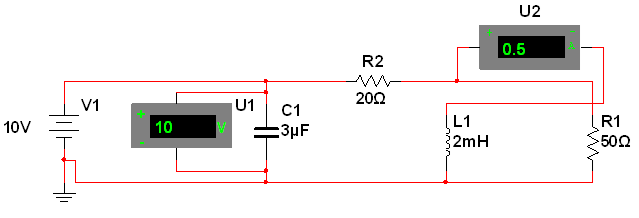
\includegraphics[width=10.82cm, height=3.68cm]{Imagenes/1.png}
	\captionof{figure}{}
\end{center}
\begin{center}
	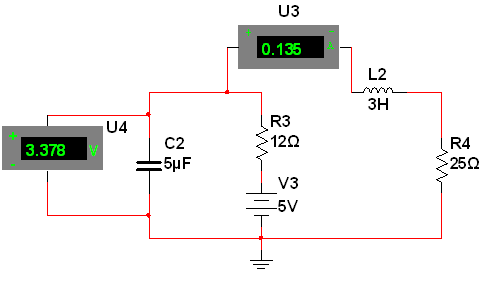
\includegraphics[width=8.26cm, height=4.83cm]{Imagenes/2.png}
	\captionof{figure}{}
\end{center}
\begin{center}
	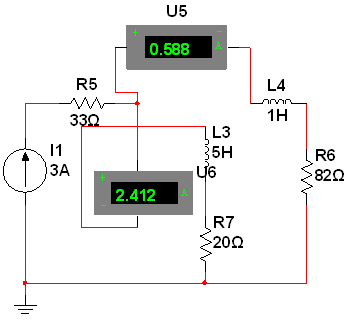
\includegraphics[width=5.97cm, height=5.59cm]{Imagenes/3.png}
	\captionof{figure}{}
\end{center}
\begin{center}
	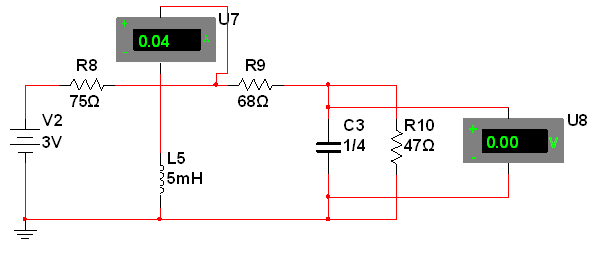
\includegraphics[width=10.08cm, height=4.32cm]{Imagenes/4.png}
	\captionof{figure}{}
\end{center}
\begin{center}
	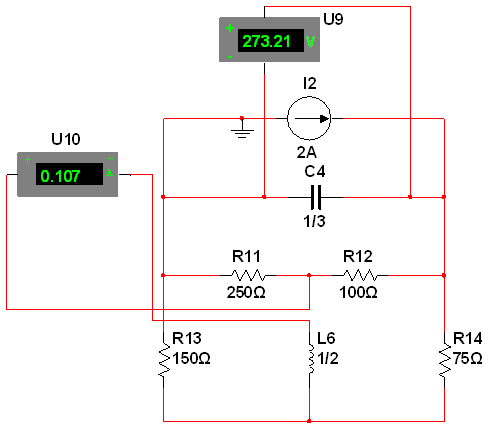
\includegraphics[width=8.32cm, height=7.22cm]{Imagenes/5.png}
	\captionof{figure}{}
\end{center}
\begin{center}
	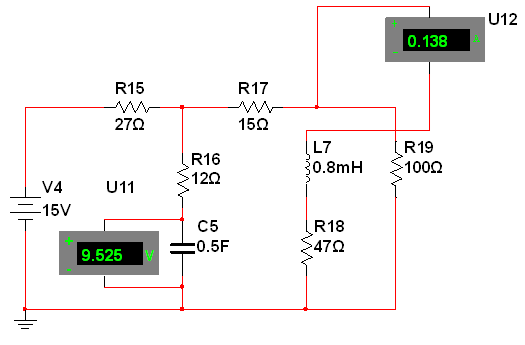
\includegraphics[width=8.89cm, height=5.84cm]{Imagenes/6.png}
	\captionof{figure}{}
\end{center}
\end{document}
